\chapter{Search for Dark Matter Annihilation in Galaxy Groups}

\noindent {\bf Introduction.}  Weakly-interacting massive particles, which acquire their cosmological abundance through thermal freeze-out in the early Universe, are leading candidates for dark matter (DM).  Such particles can annihilate into Standard Model states in the late Universe, leading to striking gamma-ray signatures that can be detected with observatories such as the {\it Fermi} Large Area Telescope.  
Some of the strongest limits on the annihilation cross section have been set by searching for excess gamma-rays in the Milky Way's dwarf spheroidal satellite galaxies (dSphs)~\cite{Ackermann:2015zua,Fermi-LAT:2016uux}.  In this Letter, we present competitive constraints that are obtained using hundreds of galaxy groups within $z\lesssim0.03$. 

This work is complemented by a companion publication in which we describe the procedure for utilizing  galaxy group catalogs in searches for extragalactic DM~\cite{companion}.  Previous attempts to search for DM outside the Local Group were broad in scope, but yielded weaker constraints than the dSph studies.  For example, limits on the annihilation rate were set by requiring that the DM-induced flux not overproduce the isotropic gamma-ray background~\cite{Ackermann:2015tah}.  These bounds could be improved by further resolving the contribution of sub-threshold point sources to the isotropic background~\cite{Zechlin:2016pme,Lisanti:2016jub}, or by  
looking at the auto-correlation spectrum~\cite{Ackermann:2012uf, Ackermann:2012uf,Ando:2006cr,Ando:2013ff}.  A separate approach involves cross-correlating~\cite{Xia:2011ax,Ando:2014aoa,Ando:2013xwa,Xia:2015wka,Regis:2015zka,Cuoco:2015rfa,Ando:2016ang} the {\it Fermi} data with galaxy-count maps constructed from, \emph{e.g.}, the Two Micron All-Sky Survey (2MASS)~\cite{Jarrett:2000me,Bilicki:2013sza}.  A positive cross-correlation was detected with 2MASS galaxy counts~\cite{Xia:2015wka}, which could arise from annihilating DM with mass $\sim$$10$--$100$~GeV and a near-thermal annihilation rate~\cite{Regis:2015zka}.  However, other source classes, such as misaligned Active Galactic Nuclei, could also explain the signal~\cite{Cuoco:2015rfa}.
  
\begin{table*}[htb]
\footnotesize
\begin{tabular}{C{3.0cm}C{2.1cm}C{1.8cm}C{1.8cm}C{1.8cm}C{1.5cm}C{1.6cm}C{1.6cm}C{1.6cm}C{1.6m}}
\toprule
\Xhline{3\arrayrulewidth}
Name &   $\log_{10} J$  &  $\log_{10} M_\text{vir}$ &          $z \times 10^{3}$&        $\ell$ &        $b$ &  $\log_{10} c_\text{vir}$ &  $\theta_\text{s}$  &  $b_\text{sh}$   \\
 & {[GeV$^2$\,cm$^{-5}$\,sr]}& [$M_\odot$] &  & [deg] & [deg] & & [deg] &\\
\midrule
\hline
            NGC4472/Virgo &  19.11$\pm$0.35 &  14.6$\pm$0.14 &   3.58 &  283.94 &  74.52 &  0.80$\pm$0.18 &     1.15 &  4.53 \\
                  NGC0253 &  18.76$\pm$0.37 &  12.7$\pm$0.12 &   0.79 &   98.24 & -87.89 &  1.00$\pm$0.17 &     0.77 &  2.90 \\
                  NGC3031 &  18.58$\pm$0.36 &  12.6$\pm$0.12 &   0.83 &  141.88 &  40.87 &  1.02$\pm$0.17 &     0.64 &  2.76 \\
        NGC4696/Centaurus &  18.33$\pm$0.35 &  14.6$\pm$0.14 &   8.44 &  302.22 &  21.65 &  0.80$\pm$0.18 &     0.47 &  4.50 \\
                  NGC1399 &  18.30$\pm$0.37 &  13.8$\pm$0.13 &   4.11 &  236.62 & -53.88 &  0.89$\pm$0.17 &     0.45 &  3.87 \\
\bottomrule
\Xhline{3\arrayrulewidth}
\end{tabular}
\caption{The top five halos included in the analysis, as ranked by inferred $J$-factor, including the boost factor.  For each group, we show the brightest central galaxy and the common name, if one exists, as well as the virial mass, cosmological redshift, Galactic longitude $\ell$, Galactic latitude $b$, inferred virial concentration~\cite{Correa:2015dva}, angular extent, and boost factor~\cite{Bartels:2015uba}.  The angular extent is defined as $\theta_\text{s} \equiv \tan^{-1} (r_\text{s} / d_c[z])$, where $d_c[z]$ is the comoving distance and $r_\text{s}$ is the NFW scale radius.  A complete table of the galaxy groups used in this analysis, as well as their associated properties, are provided at \url{https://github.com/bsafdi/DMCat}.
}
\label{Jtab}
\end{table*}

An alternative to studying the full-sky imprint of extragalactic DM annihilation is to use individual galaxy clusters~\cite{Ackermann:2010rg, Ando:2012vu,Ackermann:2013iaq,Ackermann:2015fdi,Anderson:2015dpc,Rephaeli:2015nca,2016A&A...589A..33A,Liang:2016pvm,Adams:2016alz,Huang:2011xr}. Previous analyses along these lines have looked at  
  a small number of $\sim$$10^{14}$--$10^{15}$~M$_\odot$ X-ray--selected clusters. 
  Like the dSph searches, the cluster studies have the advantage that the expected signal is localized in the sky, which reduces the systematic uncertainties associated with modeling the foregrounds and unresolved extragalactic sources.  As we will show, however, the sensitivity to DM annihilation is enhanced---and is more robust---when a larger number of targets are included compared to previous studies.

 Our work aims to combine the best attributes of the cross-correlation and cluster studies to improve the search for extragalactic DM annihilation.  We use the galaxy group catalogs in Refs.~\cite{Tully:2015opa} and~\cite{2017ApJ...843...16K} (hereby T15 and T17, respectively), which contain accurate mass estimates for halos with mass greater than $\sim$$10^{12}$~M$_\odot$ and $z \lesssim 0.03$, to systematically determine the galaxy groups that are expected to yield the best limits on the annihilation rate.  The T15 catalog provides reliable redshift estimates in the range $0.01 \lesssim z \lesssim 0.03$, while the T17 catalog provides measured distances for nearby galaxies, $z \lesssim 0.01$, based on Ref.~\cite{Tully:2016ppz}. The T15 catalog was previously used for a gamma-ray line search~\cite{Adams:2016alz}, but our focus here is on the broader, and more challenging, class of continuum signatures.  We search for gamma-ray flux from these galaxy groups and interpret the null results as bounds on the annihilation cross section.   
 
 \noindent {\bf Galaxy Group Selection.}  The observed gamma-ray flux from DM annihilation in an extragalactic halo is proportional to both the particle physics properties of the DM, as well as its astrophysical distribution:
\es{particle}{
\frac{d\Phi}{dE_{\gamma}} &= \left.  J \, \times \frac{\langle\sigma v\rangle}{8 \pi m_{\chi}^{2}} \, \, \sum_i \text{Br}_{i}\, \frac{dN_{i}}{dE'_{\gamma}} \right|_{E_{\gamma}' = (1 +z) E_{\gamma}}   \,,
}
with units of $[{\rm counts} \,\,{\rm cm}^{-2} \, {\rm s}^{-1} \, {\rm GeV}^{-1}]$.  Here, $E_\gamma$ is the gamma-ray energy, $\langle \sigma v \rangle$ is the annihilation cross section, $m_\chi$ is the DM mass, $\text{Br}_{i}$ is the branching fraction to the $i^\text{th}$ annihilation channel, and $z$ is the cosmological redshift.  The energy spectrum for each channel is described the function $dN_{i}/dE_{\gamma}$, which is modeled using PPPC4DMID~\cite{Cirelli:2010xx}.  The $J$-factor that appears in~Eq.~\ref{particle} encodes the astrophysical properties of the halo.  It is proportional to the line-of-sight integral of the squared DM density distribution, $\rho_\text{DM}$, and is written in full as 
\begin{equation}
J = \left(1+b_\text{sh}[M_\text{vir}] \right)  \int ds\,d \Omega \,\rho^{2}_\text{DM}(s,\Omega) \, ,
\label{eq:Jfactor}
\end{equation}
where $b_\text{sh}[M_\text{vir}]$ is the boost factor, which accounts for the enhancement due to substructure.  For an extragalactic halo, where the comoving distance $d_c[z]$ is much greater than the virial radius $r_\text{vir}$, the integral in Eq.~\ref{eq:Jfactor} scales as $M_{\rm vir} c_{\rm vir}^3\rho_c/d_c^2[z]$ for the Navarro-Frenk-White (NFW) density profile~\cite{Navarro:1996gj}.  Here, $M_\text{vir}$ is the virial mass, $\rho_c$ is the critical density, and $c_\text{vir}=r_\text{vir}/r_s$ is the virial concentration, with $r_s$ the scale radius.  We infer $c_\text{vir}$ using the concentration-mass relation from Ref.~\cite{Correa:2015dva}, which we update with the Planck 2015 cosmology~\cite{Ade:2015xua}.  
For a given mass and redshift, the concentration is modeled as a log-normal distribution with mean given by the concentration-mass relation.  We estimate the dispersion by matching to that observed in the \texttt{DarkSky-400} simulation for an equivalent $M_\text{vir}$~\cite{Lehmann:2015ioa}.  Typical dispersions range from $\sim$$0.14$--$0.19$ over the halo masses considered. 

The halo mass and redshift also determine the boost factor enhancement that arises from annihilation in DM substructure.  Accurately modeling the boost factor is challenging as it involves extrapolating the halo-mass function and concentration to masses smaller than can be resolved with current simulations.  Some previous analyses of extragalactic DM annihilation have estimated boost factors $\sim$$10^2$--$10^3$ for cluster-size halos (see, for example, Ref.~\cite{Gao:2011rf}) based on phenomenological extrapolations of the subhalo mass and concentration relations.  However, more recent studies indicate that the concentration-mass relation likely flattens at low masses~\cite{Anderhalden:2013wd,Ludlow:2013vxa,Correa:2015dva}, suppressing the enhancement. We use the model of Ref.~\cite{Bartels:2015uba}---specifically, the ``self-consistent" model with $M_\text{min} = 10^{-6}$~M$_\odot$---which accounts for tidal stripping of bound subhalos and yields a modest boost $\sim$$5$ for $\sim$$10^{15}$~M$_\odot$ halos. Additionally, we model the boost factor as a multiplicative enhancement to the rate in our main analysis, though we consider the effect of possible spatial extension from the subhalo annihilation in the Supplementary Material. In particular, we find that modeling the boost component of the signal as tracing a subhalo population distributed as $\rho_\text{NFW}$ rather than $\rho^{2}_\text{NFW}$ degrades the upper limits obtained by almost an order of magnitude at higher masses $m_\chi \gtrsim 500$ GeV while strengthening the limit by a small $\mathcal O(1)$ factor at lower masses $m_\chi \lesssim 200$ GeV.

The halo masses and redshifts are taken from the galaxy group catalog T15~\cite{Tully:2015opa}, which is based on the 2MASS Redshift Survey (2MRS)~\cite{Crook:2006sw}, and T17~\cite{2017ApJ...843...16K}, which compiles an inventory of nearby galaxies and distances from several sources.  The catalogs provide group associations for these galaxies as well as mass estimates and uncertainties of the host halos, constructed from a luminosity-to-mass relation. The mass distribution is assumed to follow a log-normal distribution with uncertainty fixed at 1\% in log-space \cite{companion}, which translates to typical absolute uncertainties of 25-40\%.\footnote{To translate, approximately, between log- and linear-space uncertainties for the mass, we may write $x = \log_{10} M_\text{vir}$, which implies that the linear-space fractional uncertainties are $\delta M_\text{vir} / M_\text{vir} \sim (\delta x / x) \log M_\text{vir}$. } This is conservative compared to the 20\% uncertainty estimate given in T15 due to their inference procedure. The halo centers are assumed to coincide with the locations of the brightest galaxy in the group.  We infer the $J$-factor using Eq.~\ref{eq:Jfactor} and calculate its uncertainty by propagating the errors on $M_\text{vir}$ and $c_\text{vir}$, which we take to be uncorrelated.  Note that we neglect the distance uncertainties, which are expected to be $\sim$5\%~\cite{Tully:2016ppz,2017ApJ...843...16K}, as they are subdominant compared to the uncertainties on mass and concentration.  We compile an initial list of nearby targets using the T17 catalog, supplementing these with the T15 catalog.  We exclude from T15 all groups with Local Sheet velocity $V_\text{LS} < 3000$~km s$^{-1}$ ($z \lesssim 0.01$) and $V_\text{LS} > 10,000$~km s$^{-1}$ ($z \gtrsim 0.03$), the former because of peculiar velocity contamination and the latter because of large uncertainties in halo mass estimation due to less luminous satellites.  When groups overlap between the two catalogs, we preferentially choose distance and mass measurements from T17.

The galaxy groups are ranked by their inferred $J$-factors, excluding any groups that lie within $|b| \leq 20^\circ$ to mitigate contamination from Galactic diffuse emission.  We require that halos do not overlap to within $2^\circ$ of each other, which is approximately the scale radius of the largest halos.  The exclusion procedure is applied sequentially starting with a halo list ranked by $J$-factor.  We manually exclude Andromeda, the brightest halo in the catalog, because its large angular size is not ideally suited to our analysis pipeline and requires careful individual study~\cite{Ackermann:2017nya}.  
As discussed later in this Letter, halos are also excluded if they show large residuals that are inconsistent with DM annihilation in the other groups in the sample.  Starting with the top 1000 halos, we end up with 495 halos that pass all these requirements.  Of the excluded halos, 276 are removed because they fall too close to the Galactic plane, 134 are removed by the $2^\circ$ proximity requirement, and 95 are removed because of the cut on large residuals. 

Table~\ref{Jtab} lists the top five galaxy groups included in the analysis, labeled by their central galaxy or common name, if one exists.  We provide the inferred $J$-factor including the boost factor, the halo mass, redshift, position in Galactic coordinates, inferred concentration, and boost factor.  Additionally, we show $\theta_\text{s} \equiv \tan^{-1} (r_\text{s} / d_c[z])$ to indicate the spatial extension of the halo.  We find that $\theta_\text{s}$ is typically between the 68\% and 95\% containment radius for emission associated with annihilation in the halos, without accounting for spread from the point-spread function (PSF).  For reference, Andromeda has $\theta_\text{s} \sim 2.57^\circ$.  
%A complete list of the analyzed galaxy groups is provided as Supplementary Data.

\noindent {\bf Data Analysis.}  We analyze 413 weeks of Pass 8 {\it Fermi} data in the UltracleanVeto event class, from August 4, 2008 through July 7, 2016.  The data is binned in 26 logarithmically-spaced energy bins between 502~MeV and 251~GeV and spatially with a HEALPix pixelation~\cite{Gorski:2004by} with \texttt{nside}=128.\footnote{Our energy binning is constructed by taking 40 log-spaced bins between 200~MeV and 2~TeV and then removing the lowest four and highest ten bins, for reasons discussed in the companion paper~\cite{companion}. }  The recommended set of quality cuts are applied to the data corresponding to zenith angle less than $90^\circ$, $\texttt{LAT\_CONFIG}=1$, and $\texttt{DATA\_QUAL}>0$.\footnote{\url{https://fermi.gsfc.nasa.gov/ssc/data/analysis/documentation/Cicerone/Cicerone_Data_Exploration/Data_preparation.html}.}  We also mask known large-scale structures~\cite{companion}.

The template analysis that we perform using \texttt{NPTFit}~\cite{Mishra-Sharma:2016gis} is similar to that of previous dSph studies~\cite{Ackermann:2015zua,Fermi-LAT:2016uux}  and is detailed in our companion paper~\cite{companion}.  We summarize the relevant points here.  Each region-of-interest (ROI), defined as the $10^\circ$ area surrounding each halo center, has its own likelihood.  In each energy bin, this  likelihood is the product, over all pixels, of the Poisson probability for the observed photon counts per pixel.  This probability depends on the mean expected counts per pixel, which depends on contributions from known astrophysical emission as well as a potential DM signal. Note that the likelihood is also multiplied by the appropriate log-normal distribution for $J$, which we treat as a single nuisance parameter for each halo and account for through the profile likelihood method.  

%%%%%%%%%%%%%%%%%%%%%%%%%%%  
%%%%%%%%%%%%%%%%%%%%%%%%%%%  
\begin{figure*}[t]
\centering
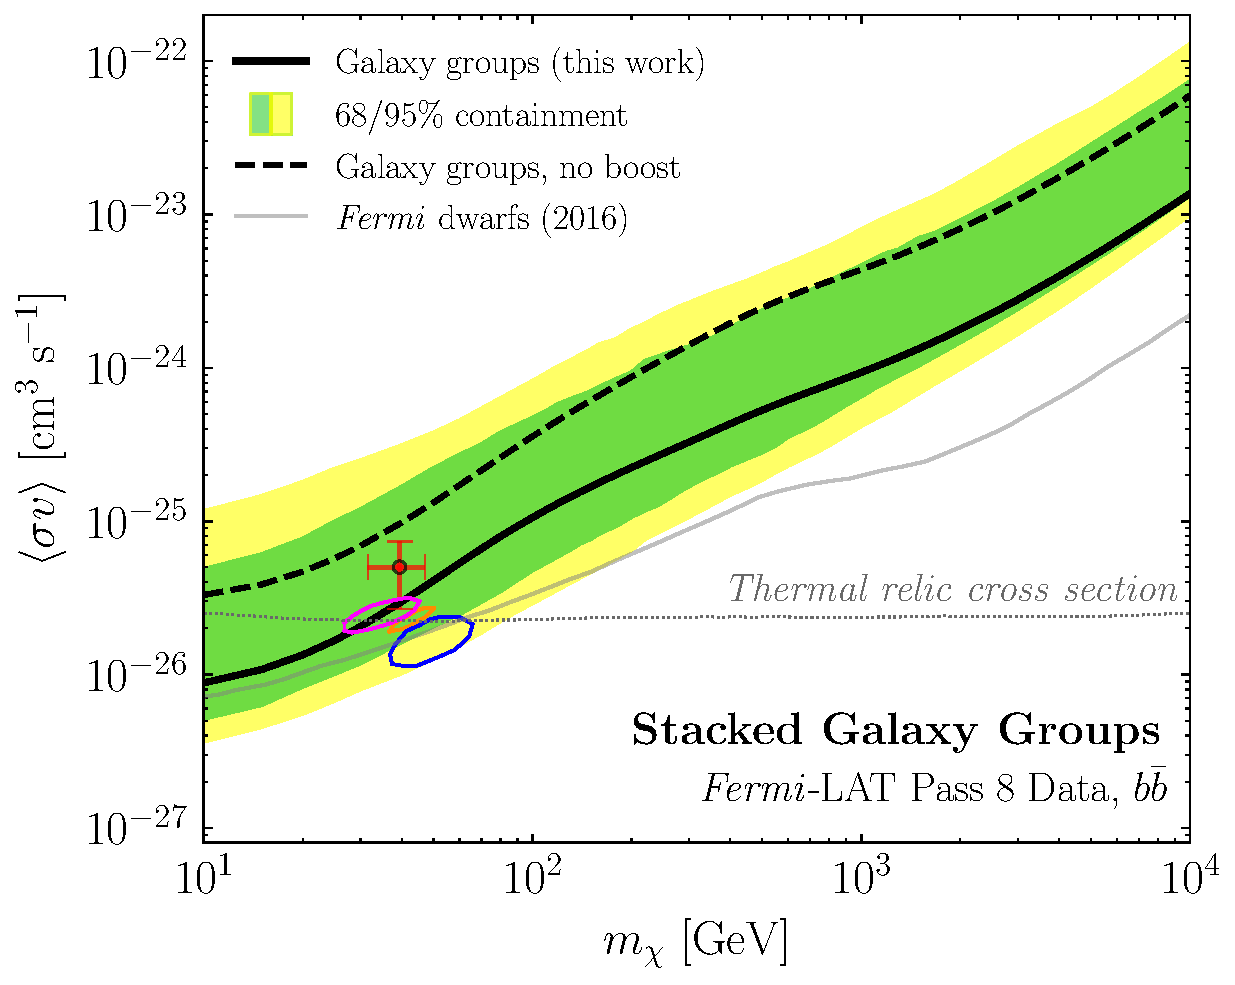
\includegraphics[width=0.45\textwidth]{ch-clusters/plots/bounds.pdf} \hspace{4mm}
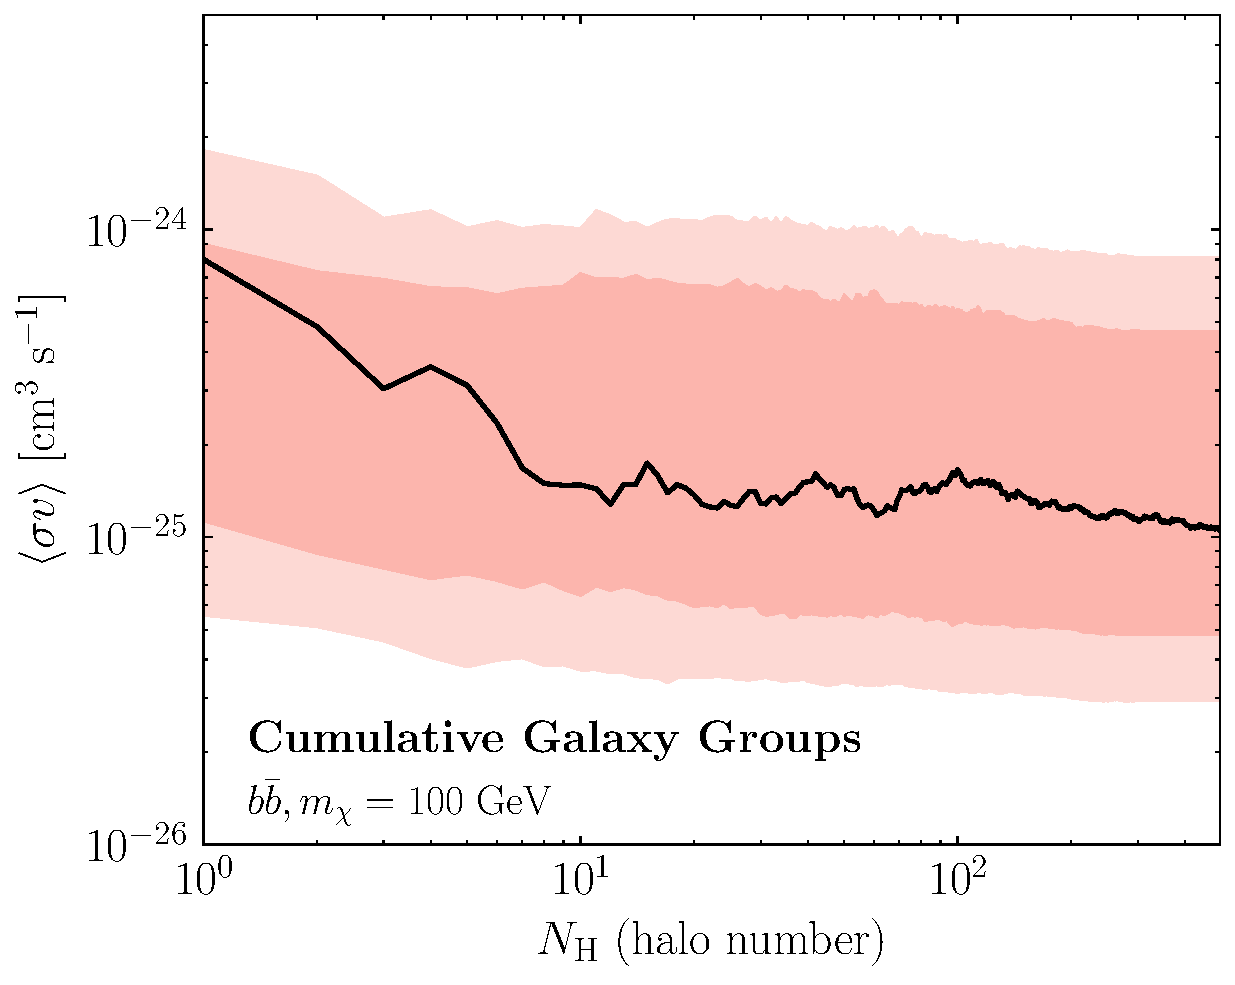
\includegraphics[width=0.45\textwidth]{ch-clusters/plots/elephant.pdf}
\caption{(Left) The solid black line shows the 95\% confidence limit on the DM annihilation cross section, $\langle \sigma v \rangle$, as a function of the DM mass, $m_\chi$, for the $b \bar b$ final state, assuming the fiducial boost factor~\cite{Bartels:2015uba}. The containment regions are computed by performing the data analysis multiple times for random sky locations of the halos.  For comparison, the dashed black line shows the limit assuming no boost factor.  The {\it Fermi} dwarf limit is also shown, as well as the $2$$\sigma$ regions where DM may contribute to the Galactic Center Excess (see text for details).  The thermal relic cross section for a generic weakly interacting massive particle~\cite{Steigman:2012nb} is indicated by the thin dotted line.   (Right) The change in the limit for $m_\chi = 100$~GeV as a function of the number of halos that are included in the analysis, which are ranked in order of largest $J$-factor.  The result is compared to the expectation from random sky locations; the 68 and 95\% expectations from 200 random sky locations are indicated by the red bands.}
\label{fig:bounds}
\end{figure*}
%%%%%%%%%%%%%%%%%%%%%%%%%%%  
%%%%%%%%%%%%%%%%%%%%%%%%%%% 

To model the expected counts per pixel, we include several templates in the analysis that trace the emission associated with: (i) the projected NFW-squared profile modeling the putative DM signal, (ii) the diffuse background, as described by the  {\it Fermi} \texttt{gll\_iem\_v06 (p8r2)} model, (iii) isotropic emission, (iv) the {\it Fermi} bubbles~\cite{Su:2010qj}, (v) 3FGL sources within $10^\circ$ to $18^\circ$ of the halo center, floated together after fixing their individual fluxes to the values predicted by the 3FGL catalog~\cite{Acero:2015hja}, and (vi) all individual 3FGL point sources within $10^{\circ}$ of the halo center.  Note that we do not model the contributions from annihilation in the smooth Milky Way halo because the brightest groups have peak flux significantly (approximately an order of magnitude for the groups in Tab.~\ref{Jtab}) over the foreground emission from Galactic annihilation and because we expect Galactic annihilation to be subsumed by the isotropic component.   

We assume that the best-fit normalizations (\emph{i.e.}, profiled values) of the astrophysical components, which we treat as nuisance parameters, do not vary appreciably with DM template normalization. This allows us to obtain the likelihood profile in a given ROI and energy bin by profiling over them in the presence of the DM template, then fixing the normalizations of the background components to the best-fit values and scanning over the DM intensity. We then obtain the total likelihood by taking the product of the individual likelihoods from each energy bin. In order to avoid degeneracies at low energies due to the large PSF, we only include the DM template when obtaining the best-fit background normalizations at energies above $\sim$$1$~GeV. At the end of this procedure, the likelihood is only a function of the DM template intensity, which can then be mapped onto a mass and cross section for a given annihilation channel. We emphasize that the assumptions described above have been thoroughly vetted in our companion paper~\cite{companion}, where we show that this procedure is robust in the presence of a potential signal.

The final step of the analysis involves stacking the likelihoods from each ROI. The stacked log-likelihood, $\log \mathcal{L}$, is simply the sum of the log-likelihoods for each ROI.  It follows that the test statistic for data $d$ is defined as
 \begin{equation}\begin{aligned}
{\rm TS}(\mathcal{M}, \langle\sigma v\rangle, m_\chi) \equiv 2 &\left[ \log \mathcal{L}(d | \mathcal{M}, \langle\sigma v\rangle, m_\chi ) \right.\\
&\left.- \log \mathcal{L}(d | \mathcal{M}, \widehat{\langle\sigma v\rangle}, m_\chi ) \right]\,,
\label{eq:TSdef}
\end{aligned}\end{equation}
where $\widehat{\langle\sigma v\rangle}$ is the cross section that maximizes the likelihood for DM model $\mathcal{M}$.    The 95\% upper limit on the annihilation cross section is given by the value of $\langle\sigma v\rangle > \widehat{\langle \sigma v\rangle}$ where $\text{TS}=-2.71$.

Galaxy groups are expected to emit gamma-rays from standard cosmic-ray processes.  Using group catalogs to study gamma-ray emission from cosmic rays in these objects is an interesting study in its own right (see, {\it e.g.}, Ref.~\cite{Jeltema:2008vu,Huber:2013cia,Ackermann:2015fdi,Rephaeli:2015nca}), which we leave to future work.  For the purpose of the present analysis, however, we would like a way to remove groups with large residuals, likely arising from standard astrophysical processes in the clusters, to maintain maximum sensitivity to DM annihilation.  This requires care, however, as we must guarantee  that the procedure for removing halos does not remove a real signal, if one were present.  

We adopt the following algorithm to remove halos with large residuals that are inconsistent with DM annihilation in the other groups in the sample. A group is excluded if it meets two conditions. First, to ensure it is a statistically significant excess, we require twice the difference between the maximum log likelihood and the log likelihood with $\langle \sigma v \rangle = 0$ to be greater than 9 at any DM mass. This selects sources with large residuals at a given DM mass.  Second, the residuals must be strongly inconsistent with limits set by other galaxy groups. Specifically, the halo  must satisfy $\langle\sigma v\rangle_\text{best} > 10 \times \langle\sigma v\rangle^*_\text{lim}$, where $\langle\sigma v\rangle_\text{best}$ is the halo's best-fit cross section at \emph{any} mass and $\langle\sigma v\rangle^*_\text{lim}$ is the strongest limit out of all halos at the specified $m_\chi$. These conditions are designed to exclude galaxy groups where the gamma-ray emission is inconsistent with a DM origin.  This prescription has been extensively tested on mock data and, crucially, does not exclude injected signals~\cite{companion}.

\noindent  {\bf Results.}  The left panel of Fig.~\ref{fig:bounds} illustrates the main results of the stacked analysis.  The solid black line represents the limit obtained for DM annihilating to a $b \bar b$ final state using the fiducial boost factor model~\cite{Bartels:2015uba}, while the dashed line  shows the limit without the boost factor enhancement.  To estimate the expected limit under the null hypothesis, we repeat the analysis by randomizing the locations of the halos on the sky 200 times, though still requiring they pass the selection cuts described above.  
The colored bands indicate the 68 and 95\% containment regions for the expected limit.  
The limit is consistent with the expectation under the null hypothesis.

The right panel of Fig.~\ref{fig:bounds} illustrates how the limits evolve for the $b \bar b$ final state with $m_\chi = 100$~GeV as an increasing number of halos are stacked.  We also show the expected 68\% and 95\% containment regions, which are obtained from the random sky locations.  As can be seen, no single halo dominates the bounds.  For example, removing Virgo, the brightest halo in the catalog, from the stacking has no significant effect on the limit.  Indeed, the inclusion of all 495 halos buys one an additional order of magnitude in the sensitivity reach.

The limit derived in this work is complementary to the published dSph bound~\cite{Ackermann:2015zua,Fermi-LAT:2016uux}, shown as the solid gray line in the left panel of Fig.~\ref{fig:bounds}. Given the large systematic uncertainties associated with the dwarf analyses (see~\emph{e.g.}, Ref.~\cite{Geringer-Sameth:2014qqa}), we stress the importance of using complementary targets and detection strategies to probe the same region of parameter space. Our limit also probes the parameter space that may explain the Galactic Center excess (GCE); the best-fit models are marked by the orange cross~\cite{Abazajian:2014fta}, blue~\cite{Calore:2014xka}, red~\cite{Gordon:2013vta}, and orange~\cite{Daylan:2014rsa} $2$$\sigma$ regions.  The GCE is a spherically symmetric excess of $\sim$GeV gamma-rays observed to arise from the center of the Milky Way~\cite{Goodenough:2009gk,Hooper:2010mq,TheFermi-LAT:2015kwa,Karwin:2016tsw}.  The GCE has received a considerable amount of attention because it can be explained by annihilating DM.  However, it can also be explained by more standard astrophysical sources; indeed, recent analyses have shown that the distribution of photons in this region of sky is more consistent with a population of unresolved point sources, such as millisecond pulsars, compared to smooth emission from DM~\cite{Lee:2015fea, Bartels:2015aea,Linden:2016rcf, FermiLAT:2017yoi}.  Because systematic uncertainties can be significant and hard to quantify in indirect searches for DM, it is crucial to have independent probes of the parameter space where DM can explain the GCE.  While our null findings do not exclude the DM interpretation of the GCE, their consistency with the dwarf bounds put it further in tension.  This does not, however, account for the fact that the systematics on the modeling of the Milky Way's density distribution can potentially alleviate the tension by changing the best-fit cross section for the GCE.   

\noindent  {\bf Conclusions.} This Letter presents the results of the first systematic search for annihilating DM in nearby galaxy groups.  We introduced and validated  a prescription to infer properties of DM halos associated with  these groups, thereby allowing us to build a map of DM annihilation in the local Universe.  Using this map, we performed a stacked analysis of several hundred galaxy groups and obtained bounds that exclude thermal cross sections for DM  annihilating to $b \bar b$ with mass below $\sim$$30$~GeV, assuming a conservative boost factor model.  These limits are competitive with those obtained from the \emph{Fermi} dSph analyses and are in tension with the range of parameter space that can explain the GCE.  Moving forward, we plan to investigate the objects with gamma-ray excesses to see if they can be interpreted in the context of astrophysical emission.  In so doing, we can also develop more refined metrics for selecting the optimal galaxy groups for DM studies.    

%We include Supplementary Material that further extends the results presented here.  There, we show limits for additional annihilation final states and the brightest individual halos.  We also show how the limits are affected by several analysis choices, such as the inclusion of Andromeda and Virgo, as well as a variety of systematic uncertainties.  A complete table of the galaxy groups used in this analysis, as well as their associated properties, are provided in Supplementary Data, which can be accessed at \url{https://github.com/bsafdi/DMCat}.  The catalog includes decay factors for all of the groups in addition to the annihilation $J$-factors.  We emphasize that the supplementary catalog is separate from the {\it Fermi} analysis presented here and may be used to search for extragalactic DM annihilation and decay into neutral cosmic rays, regardless of wavelength, messenger, and instrument.

\noindent{\textbf{Acknowledgements.}  We thank S.~Ando, N.~Bahcall, R.~Bartels, J.~Beacom, P.~Behroozi, F.~Calore, W.~Coulton, A.~Drlica-Wagner, D.~Hooper, S.~Horiuchi, A.~Kravtsov, T.~Linden, Y.~Mao, K.~Murase, L.~Necib, J.~Ostriker, A.~Peter, T.~Slatyer, B.~Tully, R.~Wechsler, C.~Weniger, and S.~Zimmer for helpful conversations. This research made use of the \texttt{Astropy}~\cite{2013A&A...558A..33A}, \texttt{IPython}~\cite{PER-GRA:2007}, \texttt{Minuit}~\cite{James:1975dr}, and \texttt{NPTFit}~\cite{Mishra-Sharma:2016gis} software packages.  
ML is supported by the DOE under contract DESC0007968, the Alfred P.~Sloan Foundation and the Cottrell Scholar Program through the Research Corporation for Science Advancement.  
NLR is supported by the DOE under contracts DESC00012567 and DESC0013999.
BRS is supported by a Pappalardo
Fellowship in Physics at MIT.  This work was performed in part at Aspen Center for Physics, which is supported by NSF grant PHY-1607611.